\setcounter{secnumdepth}{1} % or 2 for numbered sections, or whatever
\setcounter{chapter}{0}

\addtocontents{toc}{\protect\setcounter{tocdepth}{1}}
\chapter*{APÊNDICE A - DOCUMENTO DE PROCESSO}\label{apendice_processo}
\addcontentsline{toc}{chapter}{APÊNDICE A - DOCUMENTO DE PROCESSO}
\addtocontents{toc}{\protect\setcounter{tocdepth}{-1}}

\begin{figure}[H]
\centering
\caption[caption]{Processo Desenvolvido}
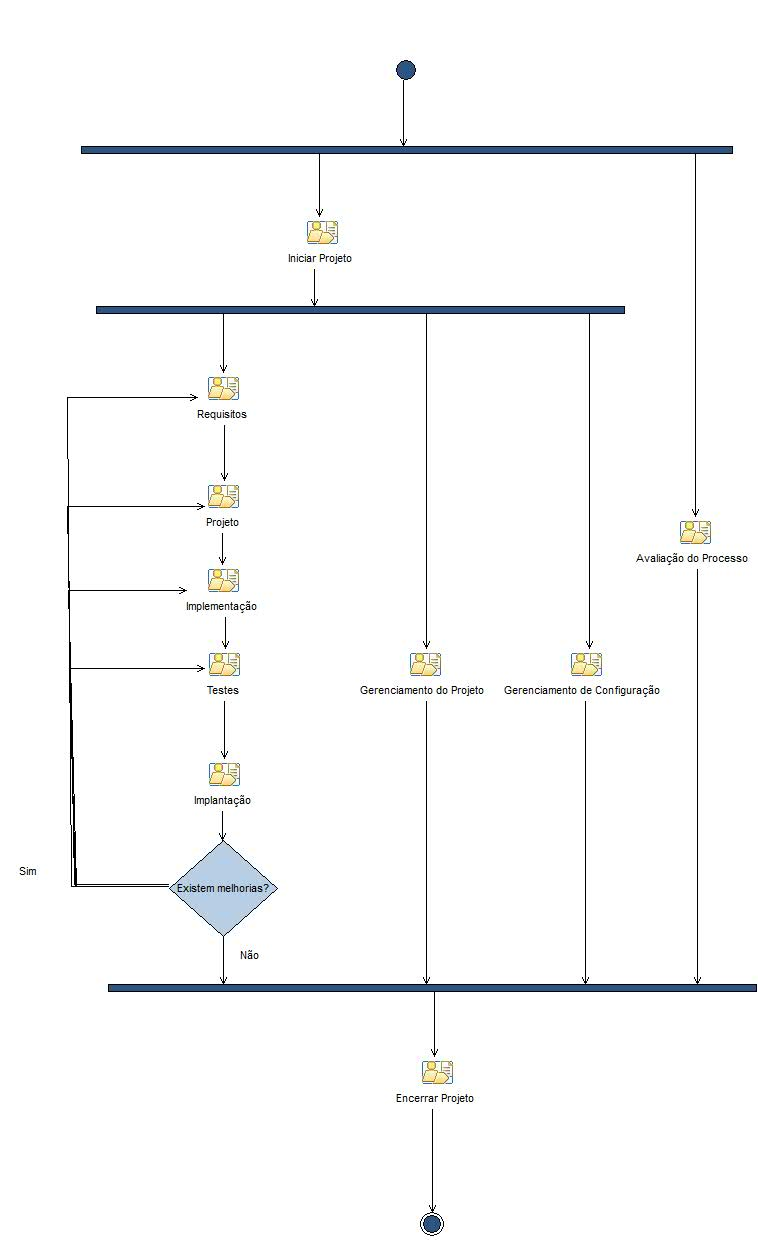
\includegraphics[width=10cm]{figuras/figura_processo}
\label{figura_processo}
\fnote{Disponível em: \url{www.askmath.quixada.ufc.br/static/process/}}
\end{figure}